\documentclass[]{article}

\title{Flow-induced shape reconfiguration in houseplants}
\author{C Smith}
\date{\today}

\usepackage{siunitx}
\usepackage{graphicx}
\usepackage[round,authoryear]{natbib}
\bibliographystyle{apalike}
\usepackage[plain]{fancyref}
\usepackage{listings}
\usepackage{amsmath,amsfonts,amssymb}
\usepackage{booktabs}
\begin{document}
\lstset{
  basicstyle=\ttfamily}https://www.overleaf.com/project/5e8d4ee557c7af0001313402



\maketitle
\begin{abstract}
	This study was conducted to investigate how effectively citrus plants can change their structure to generate less drag in wind. A cord with known spring constant was attached to a young grapefruit plant and an aluminum model of one of its leaves, a box fan was used to create a wind tunnel, and area was calculated using Matlab's color thresholding and blob detection software. The actual drag created on the grapefruit leaves was significantly less than the drag expected on an identical model, and slow motion video analysis indicated that this was the result of the citrus's ability to bend at the petiole. The extreme bending in several directions showed the plant's possible inclination toward protective load shedding.
    
\end{abstract}

\section{Introduction}
%Smith: The main ones to look at closely are Vogel and also Laura Miller and Company, and then the algae stuff from Emily Carrington, Mark Denny, Hannah Stewart, etc. May also search on ecological safety factors, reconfigurable structures, use of physical models. I didn't check mangrove literature for drag and shape reconfiguration, I think there's also coral literature about corals breaking during hurricanes to reduce loads / save the colony from death. In engineering context, this is same idea as protective load shedding in electrical systems, or crumple zones and holding bulkheads in structural systems; reefing during sailing, etc. 
	Plants possess unique structural designs and material properties which allow them to combat the negative effects of drag in their environments. As explained by \citep{delangre,2008}, fluid flow over plant canopies creates a drag force on the structure through both pressure difference and friction. In the classic drag equation, both of these factors are combined into the singular drag coefficient, creating the relationship
\[F=0.5*CpV^2A\]where \textit{F} is the total drag force, \textit{C} is the drag coefficient, \textit{p} is the fluid density, \textit{V} is relative fluid velocity, and \textit{A} is the cross-sectional area of the surface normal to the flow direction. As found by \citep{vogel,1989}, plants use their flexible structures to reconfigure under drag load, rolling their leaves into cones in order to minimize cross sectional area, drag coefficient, and the oscillations of vortex shedding. This allows plants to endure the onslaught of heavy winds or floodwaters with much lower risk for structural damage than if they were to be entirely rigid. 
	However, there is room for over correction. As shown in simulations by \citep{miller, et al,2012}, the presence of a flexible tether on the leaves, such as their stems, results in increased vortex shedding, causing much more erratic fluttering and increased drag forces. For this reason, plants are left to vary in levels of rigidity in their leaf stems in an effort to minimize drag while also avoiding excessive vortex shedding. 
    One specimen of interest in this struggle is \emph{Citrus x paradisi} (grapefruit), whose winged petioles exhibit a jointed structure. It is possible that such a structure presents a balance between the counterproductive rigidity found by Miller, et al, as it combines the rigid nature of the petiole itself with the flexible nature of a joint. The purpose of this study is to investigate the effectiveness of this petiole structure when compared to a structure lacking in all flexibility.

\section{Methods and materials}
\begin{itemize}
\item 1 six-year old grapefruit plant
\item 1 cord of known spring constant
\item 1 measuring tape
\item 1 Kaz Inc. Ht-908 15 inch Honeywell Turbo Force Room Air Circulator Fan
\item colored construction paper
\item 1 pair of scissors
\item clear tape
\item 1 Samsung Galaxy S-8 smartphone camera
\item 1 wooden chair
\item flat, rectangular surfaces
\item MATLAB software
\item pipe cleaners
\item nylon rope
\end{itemize}

	The first step in the process was to find a cord of known spring constant. In this experiment, a cord from a party mask was found to have a spring coefficient of 1.03 N/cm. The cord was attached to a nylon rope and tied to pipe cleaners at both ends so that it could be connected to plant stems. The pipe cleaners were included in the spring constant calculation.

	The experimental setup for measuring the spring's deflection due to drag is shown in Figure 1. The cord was strung between a heavy chair and the trunk of a grapefruit plant so that it was not slack, and its length was measured using a tape measure. Then, a box fan was placed one foot away from the trunk of the plant. The plant and fan were raised using flat, rectangular objects, such as textbooks, in order to position the plant's canopy in front of the fan. The cord's deflection was measured five times at each of the fan's three speed settings and a slow motion video of the plant's leaves was taken at the highest fan setting.

	Next, the cross sectional area of the plant was calculated using color blob detection in Matlab. To do this, black construction paper was cut to the size and shape of the fan's opening and affixed to it. Because air was blowing from relatively close to the plant, only the area which was directly in front of the fan opening would be exposed to wind. The plant was of a complex shape, so it was more efficient to calculate the area of the fan which was not covered by the plant. The setup was photographed from afar and scaled to eliminate the colorful surroundings, as shown in Appendix 1. A picture of the fan-shaped paper was also taken against a blue background from the same distance with no citrus obscuring it and scaled by the same amount, which can also be seen in Appendix 1. Using Matlab's colorThresholder system, the ratio of covered to uncovered area was found and multiplied by the known paper area to find the area of the grapefruit leaves.

	After analyzing the results of the grapefruit plant, a rigid model of a single leaf was created to test the same conditions without the presence of bending. A small leaf was placed against an aluminum Chipotle bowl lid to serve as a stencil, which was cut out using scissors. Then, this model leaf was taped to a wooden pencil so that the pencil would prevent it from flexing, while any tape edges were cut off. The finished leaf model can be seen in 
Figure 2.

	The leaf model was tested in the same manner as the grapefruit plant at the highest fan setting. Because the deflection in the cord was quite small, the displacement was measured using slow motion video. To do this, a tape measure with millimeters marked was taped below the cord and the video was taken from directly above. The video device was planted on a solid surface to minimize movement, and the displacement was found by zooming in on the video and pausing when the cord was fully extended and relaxed. The experimental setup for the model can be seen in Figure 3.

	In order to compare the model area to the area of the grapefruit, a sheet of orange construction paper was photographed with and without the model leaf against it. Then, using the color blob detection technique in Matlab, the ratio of the model area to the paper area was calculated and multiplied by the actual paper area, in square feet. The images for this analysis can be seen in Appendix 2.

	With the approximate cross sectional areas of the actual grapefruit leaves and the model found, the discussion over how these areas and their corresponding drags differed could begin.


% Fig 1 is good but cluttered, can we zoom in on only the business part; or turn it into a drawing. Altnatively, add callouts and scale bar? Is there a shot more from the side, that shows the experimental rig without foreshortening? 
% Agreed, I'll put in a drawing instead to make it neater
\begin{figure}
\begin{center}
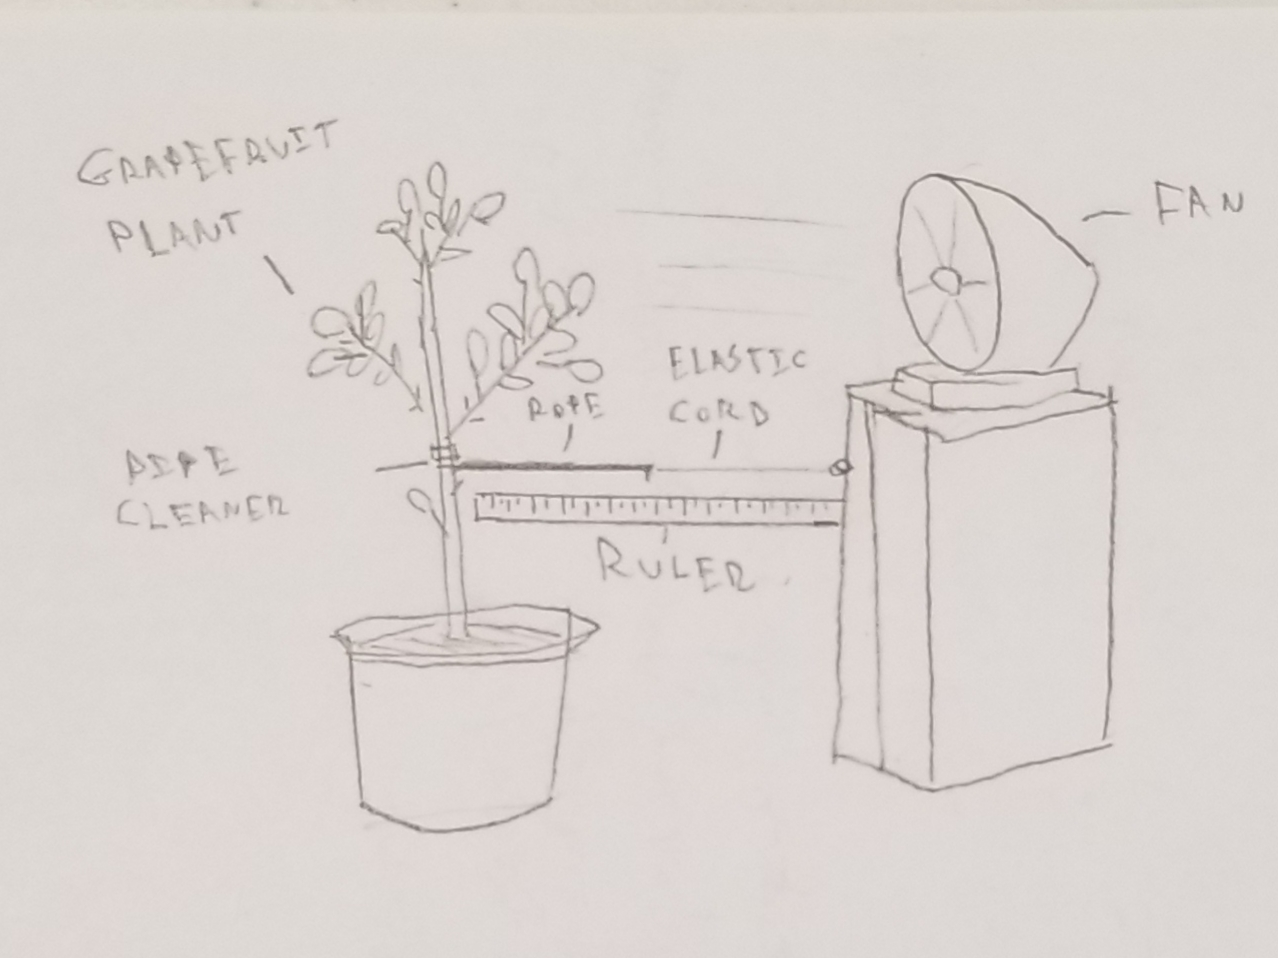
\includegraphics[width=0.5\columnwidth]{Setup1.jpg} 
\end{center}
\caption{Experimental setup to measure the deflection of a grapefruit plant when exposed to wind.}
\label{fig:methods1}
\end{figure}

% Fig 2 is good but zoom in on the two, add callouts and a scalebar, maybe rotate leaves into their normal positions. 
\begin{figure}
\begin{center}
\includegraphics[width=0.33\columnwidth]{Metal_Leaf_Compared.jpg}
\includegraphics[width=0.33\columnwidth]{Measured Model.jpg}
\end{center}
\caption{The aluminum grapefruit leaf model (left) with a small jackfruit leaf. Measuring tape (cm) along the model, for scale (right).}
\label{fig:methods2}
\end{figure}

\begin{figure}
\begin{center}
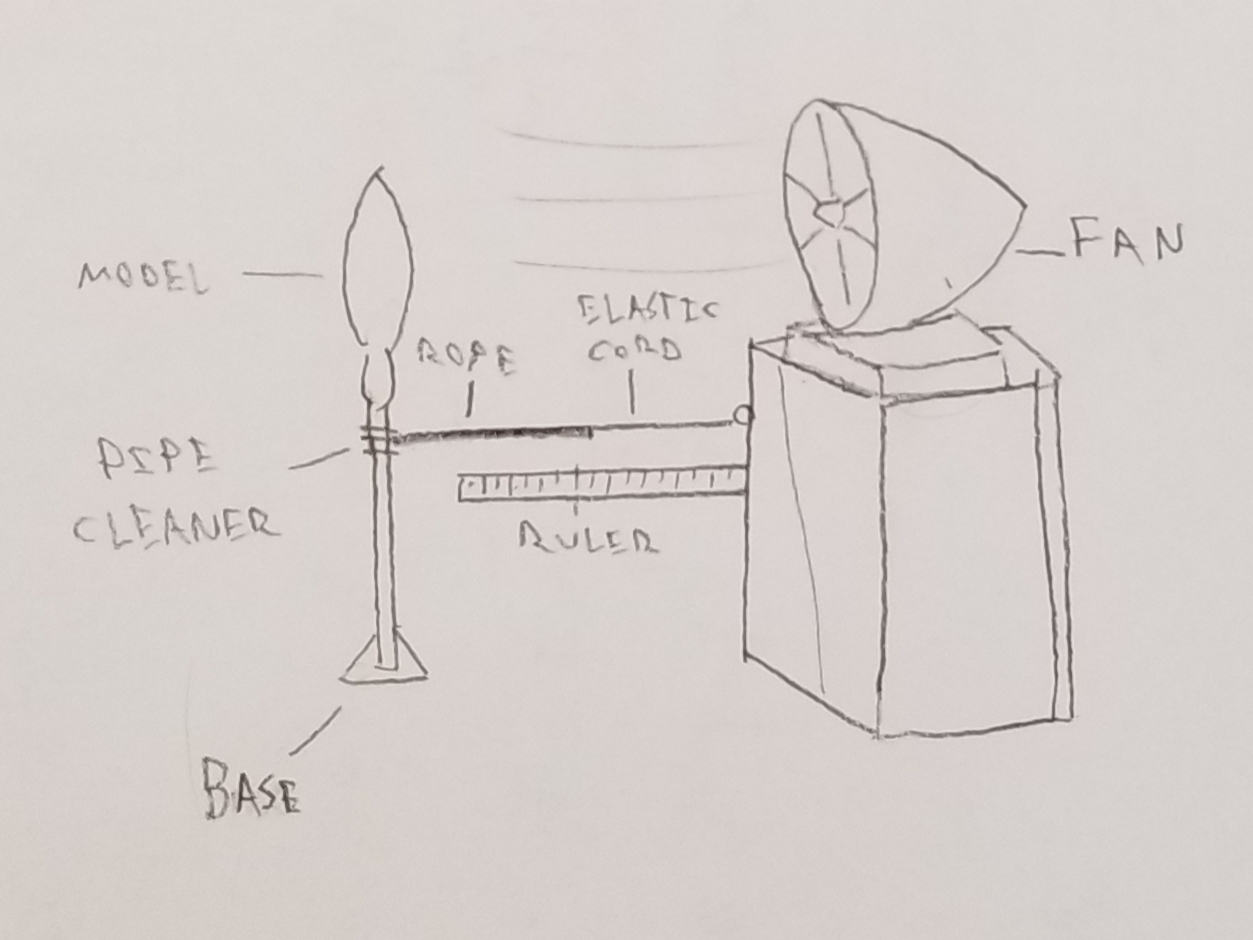
\includegraphics[width=0.5\columnwidth]{Setup2.jpg}
\end{center}
\caption{The setup for testing the rigid model drag when exposed to wind.}
\label{fig:methods3}
\end{figure}




\subsection{Specimens and physical models}
	I used a single \SI{6}{y} old specimen of \emph{Citrus x paradisi} (grapefruit) for all measurements. This specimen was germinated in Toledo, Ohio in January of 2014. As it grew, it spent its summers in the bright outdoors and winters in the relatively dark indoors, staying in a plastic pot throughout its life. This caused it to grow top heavy, with larger leaves in the canopy and smaller leaves in its understory. Additionally, it was subject to attacks from Tetranychidae (spider mites) each winter, leaving many leaves scarred. At the time of these trials, the specimen had just ended its winter indoor period, causing it to experience rapid growth. It stood at \SI{41}{in} tall and measured \SI{25}{in} across at its widest point. The wind tunnel analysis was focused on the plant's disproportionately large top.

	To remove the effects of flexibility, I also created a physical model of a single \emph{C. x paradisi} leaf using \SI{0.1}{mm} thick aluminum sheeting from a food container (Chipotle; 6658 Airport Hwy ste c, Holland, OH 43528). To prepare the physical model, I traced an actual leaf and cut the profile of the model to match. The physical model was mounted on a wooden pencil to provide a rigid attachment point compared to the typical flexible leaf petioles on \emph{C. x paradisi}. The finished product can be seen in Figure 2.

\subsection{Measurements}

\begin{table}

\caption{Average measured force and area.}

\label{tbl:results1}
\begin{center}
Average force (\si{lbf})\\
\begin{tabular}{cccc}
\toprule
grapefruit & grapefruit & grapefruit & metal leaf \\
speed 1 & speed 2 & speed 3 & speed 3 \\
\midrule
0.051 & 0.061 & 0.79 & 0.014\\
\bottomrule
\end{tabular}
\end{center}
\begin{center}
Area data (\si{ft\squared})\\
\begin{tabular}{cc}
\toprule
grapefruit & metal leaf \\
\midrule
208 & 32.8 \\
\bottomrule
\end{tabular}
\end{center}
\end{table}

\subsection{Statistical analyses}
Statistical analyses of the effects of both leaf and fan speed on drag and drag/area were performed using R \citep{r2020} using two-way analysis of variance (ANOVA); plots were prepared using the \lstinline{tidyverse} and \lstinline{ggplot2} libraries \citep{wickham2019tidyverse}.

Applying the percent difference formula

\[D=100*\frac{2*|V1-V2|}{|V1-V2|}\]
yields a difference of 17 percent between the drag to area ratios of the model and the actual plant at fan setting 3. 

\section{Results}
%Explain factually what you found... leave interpretation of what it means for the final discussion section. Here you would include plots of what you found or comparison tables.
% Qualitatively, are there photos showing how the grapefruit leaves moved under wind? Did they bend in particular places, or fold up or rotate in particular ways to reduce their drag?
\begin{tabular}{ccccc}
      & grapefruit & grapefruit & grapefruit & model \\
      & speed 1 & speed 2 & speed 3 & speed 3 \\
     Average Drag/Area & 0.00024 & 0.00029 & 0.00038 & 0.00045

\end{tabular}
\begin{figure}
    \centering
    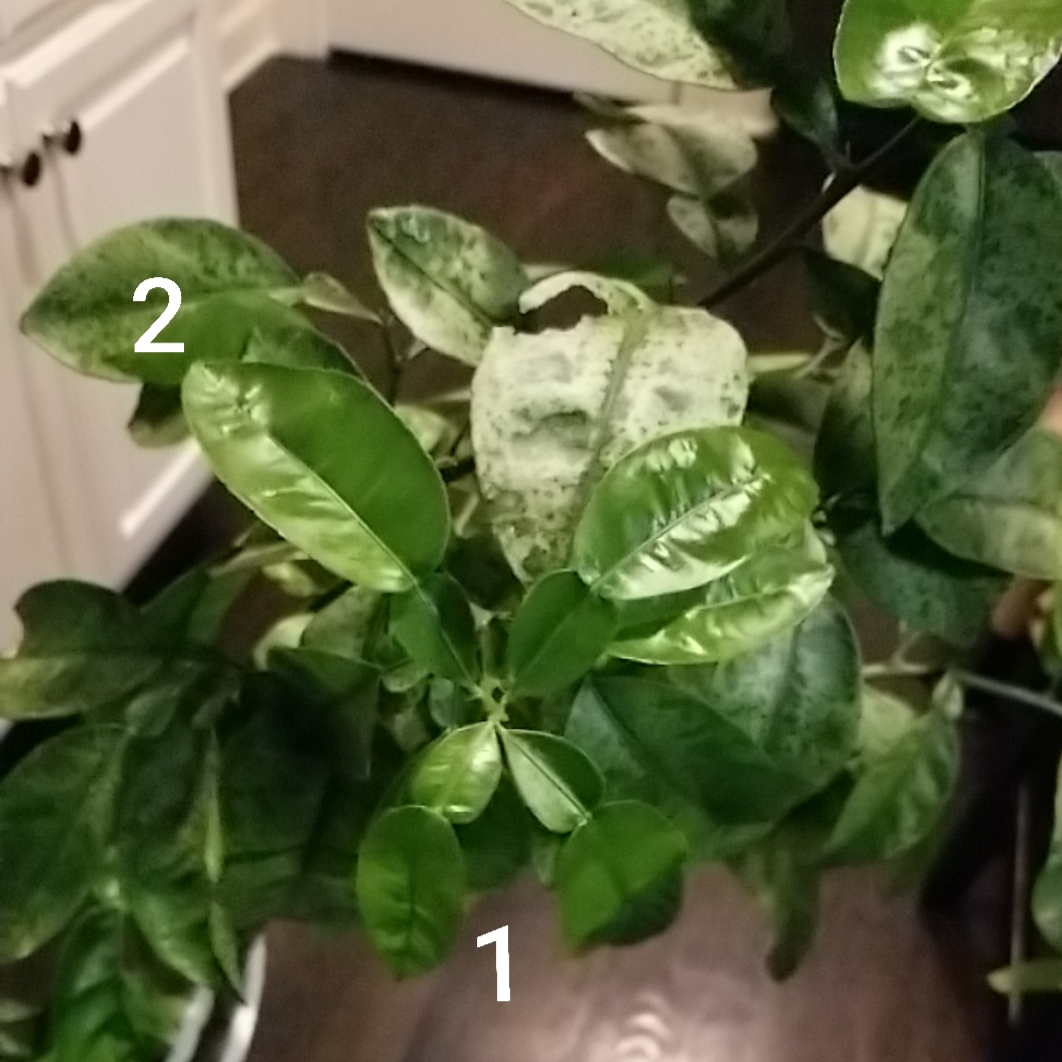
\includegraphics{Snapshot1.jpg}
    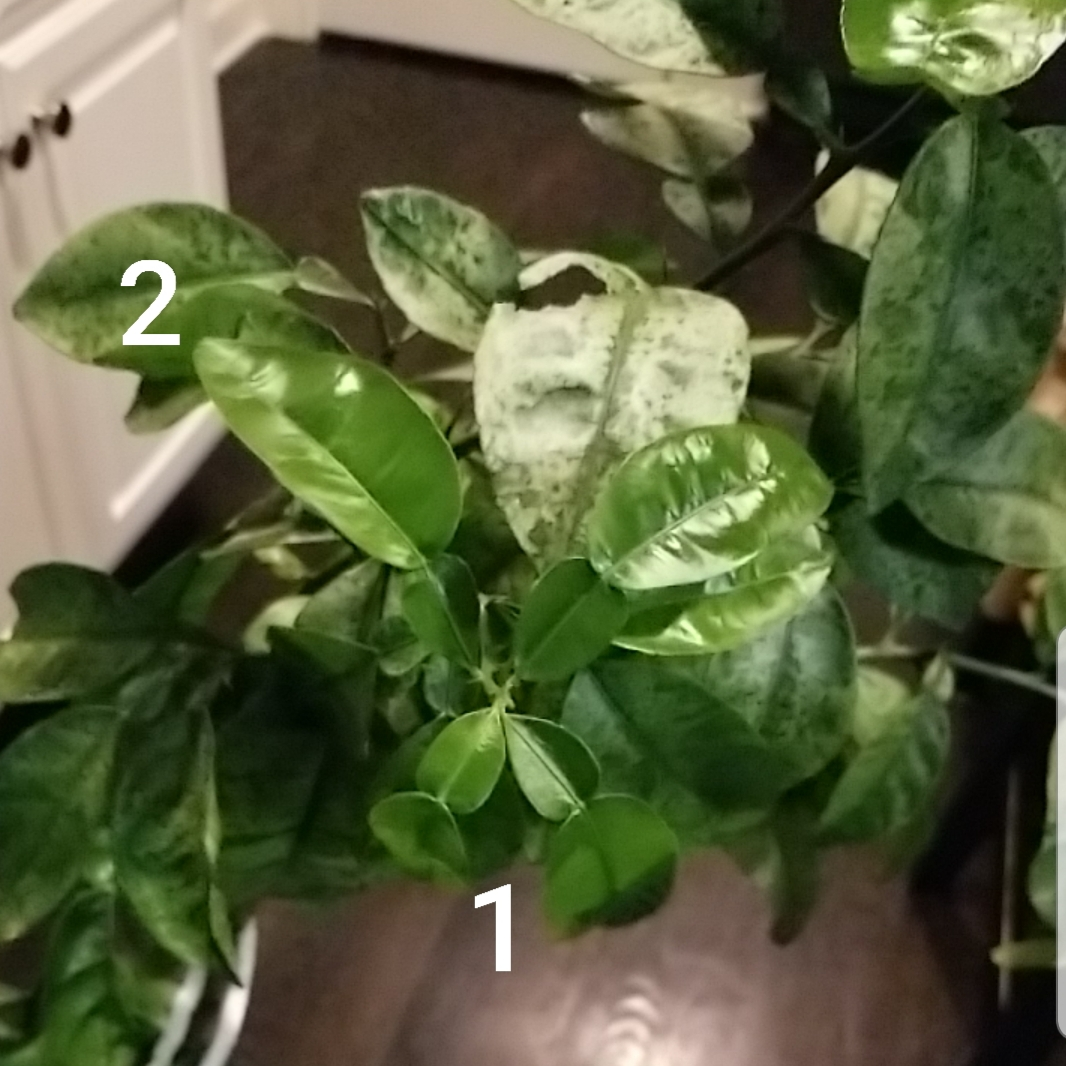
\includegraphics{Snapshot2.jpg}
    \caption{Caption}
    \label{fig:results1}
\end{figure}
\begin{figure}
    \centering
    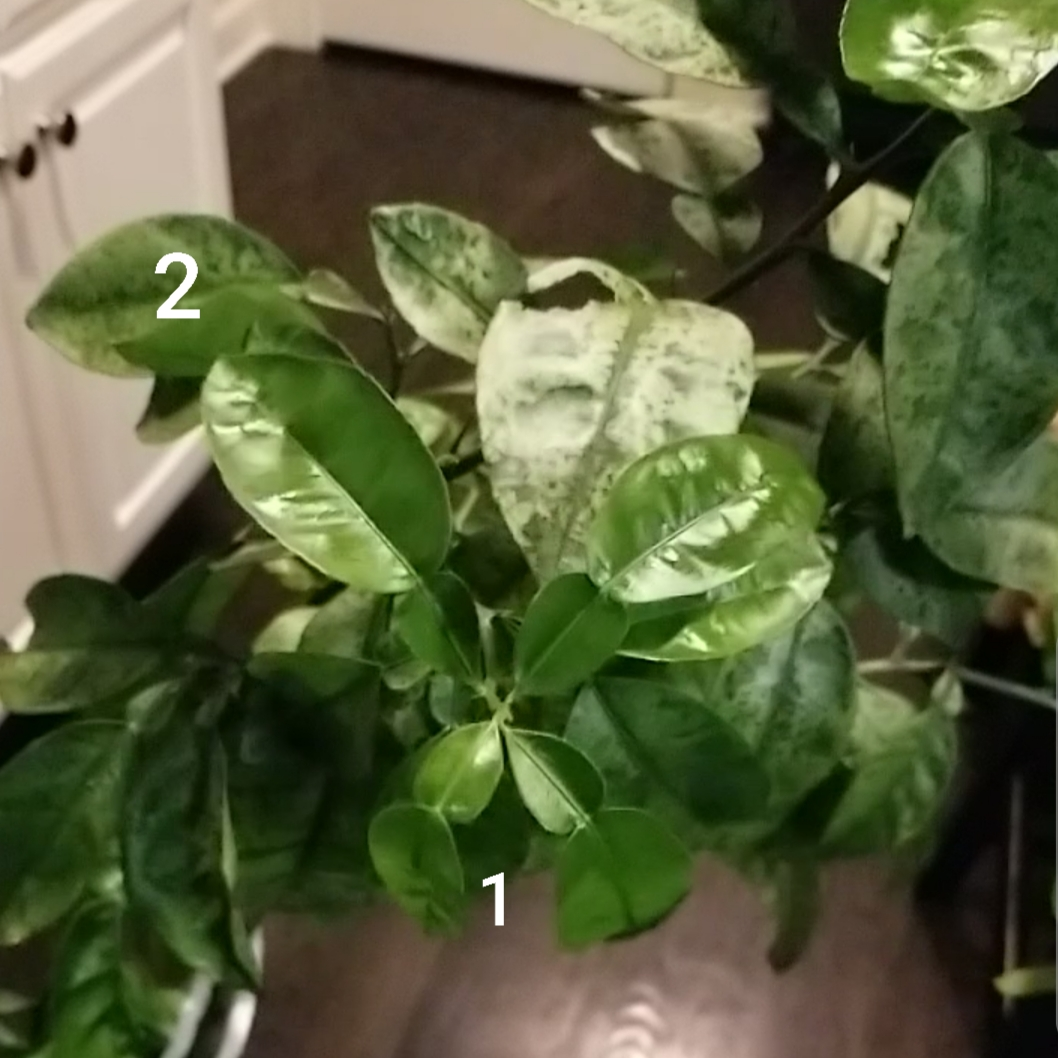
\includegraphics{Snapshot3.jpg}
    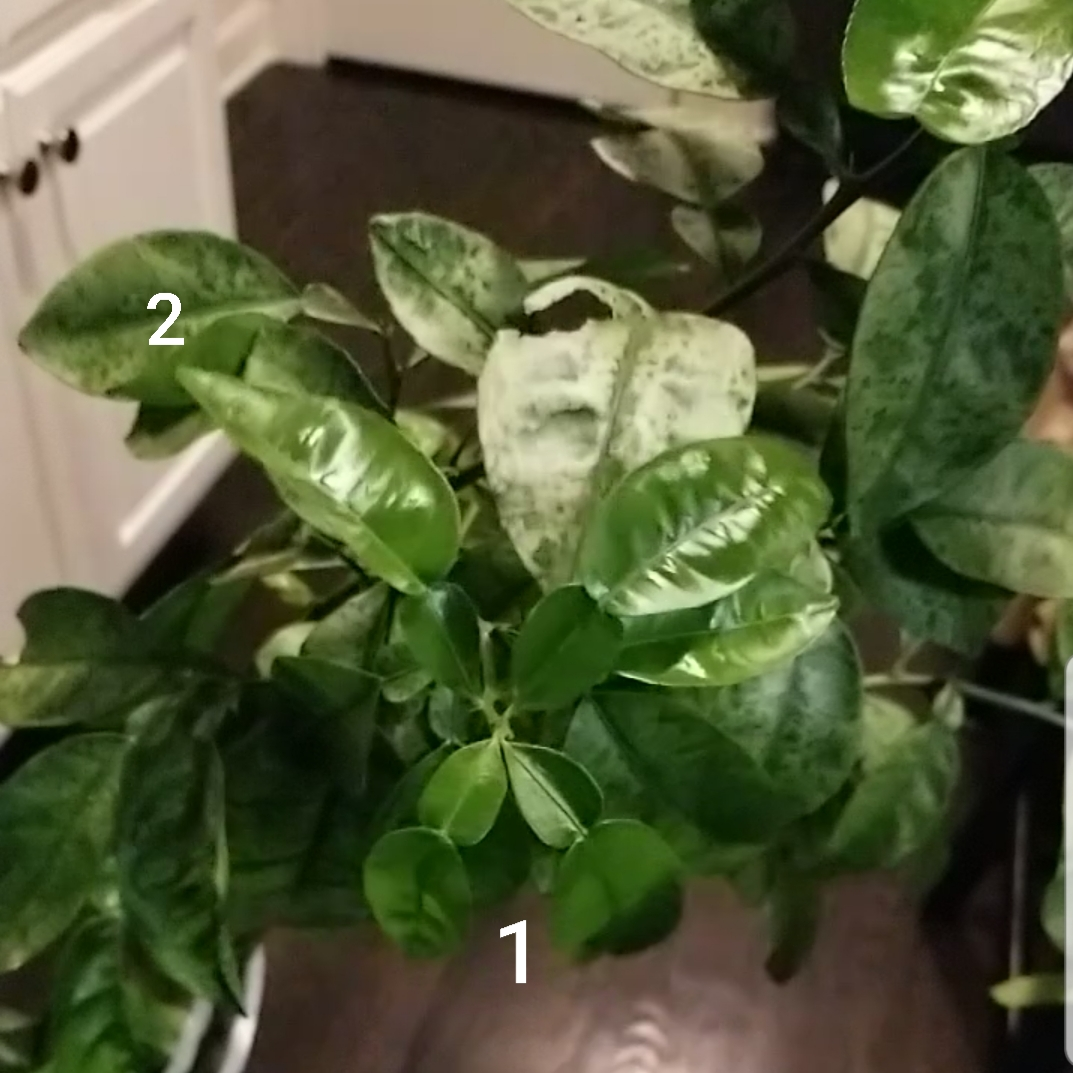
\includegraphics{Snapshot4.jpg}
    \caption{Caption}
    \label{fig:results2}
\end{figure}
	Figures 4 and 5 both show frames from the slow motion video of the \emph{C. x paradisi} leaves in the wind. Following the leaves indicated by the number 1, the leaves which were struck head-on by the wind flexed quite far at their joints, exposing roughly half of their surface area to the camera. The leaf indicated with the number 2 in Figure 5 shows the continued vortex shedding on the leaves when wind was blown across them. The leaf pivoted at its joint, but only exposed about half of its area to the wind before returning to its previous state.

\Fref{fig:results1} shows... (what does it show). When the drag is normalized by area, the effect of leaf flexibility is apparent. \Fref{fig:results2} shows... (what does it show). 

\begin{figure}
\begin{center}
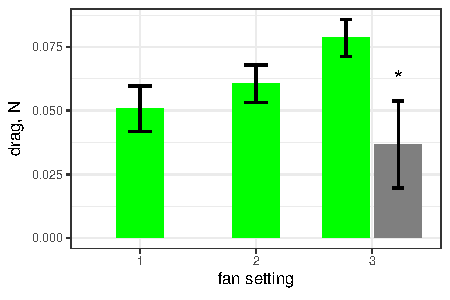
\includegraphics{data/results1.pdf}
\end{center}
\caption{Drag (mean$\pm$sd) for grapefruit (green) and metal (gray) leaves at different fan speeds. The smaller model metal leaf has less drag than the actual grapefruit leaves because of smaller area (two-way ANOVA, $p<\num{1.67e-5}$, $n=5$).}
\label{fig:results1}
\end{figure}

\begin{figure}
\begin{center}
\includegraphics{data/results2.pdf}
\end{center}
\caption{Drag, normalized by area, (mean$\pm$sd) for grapefruit (green) and metal (gray) leaves at different fan speeds. Normalized by area, the rigid metal leaf has significantly more drag than the flexible grapefruit leaves at low speeds and at the highest speed (two-way ANOVA, $p<0.003$, $n=5$).}
\label{fig:results2}
\end{figure}


\section{Discussion}
	The drag to area ratio showed the effectiveness of the petiole joints numerically, while the slow-motion video analysis suggests the reason behind the statistically significant results. This relationship implies a disposition to protective load shedding in \emph{C. x paradisi}.
	The 17 percent difference between the model drag to area ratio and that of the actual plant indicate that the leaf petioles did indeed decrease the amount of drag experienced by the plant. As the slow motion video showed, the leaves were able to bend quite far at their joints before further deforming to reduce drag. They also avoided rapid flapping through the rigidity offered by the petioles. It would appear that the petioles gave the leaves a pivot point which allowed them to reposition effectively, but the petioles' firm connections to the stem kept the leaves from experiencing the complex fluttering observed by Miller, et al.
    The drag measurements were taken from a point halfway down the trunk of the plant and the model, and therefore did not capture the torque experienced by the petiole joints. Judging from the immense range of motion in all three axes shown in the slow motion videos, it is reasonable to assume that the leaves' movements produced disproportionately large torque on their petiole joints, while producing significantly less drag on the entire plant when compared to a rigid model. This nature implies that the petiole joints are more likely to give under stress before the plant itself is uprooted or a branch detached. While more official studies will need to be made to quantify the torque on the petiole joints, I can say from personal experience, as the plant's caretaker, that high winds in the spring have taken off several large leaves on this specific specimen, with the petiole being their consistent fracture point. The joints thus play a dual function, reducing the plant's overall drag while also reducing the negative effects of fluttering to the leaves themselves, rather than the plant, as a whole.

\section{Acknowledgements}

% References
\bibliography{smith.bib}

\clearpage
\appendix
\begin{figure}
\begin{center}
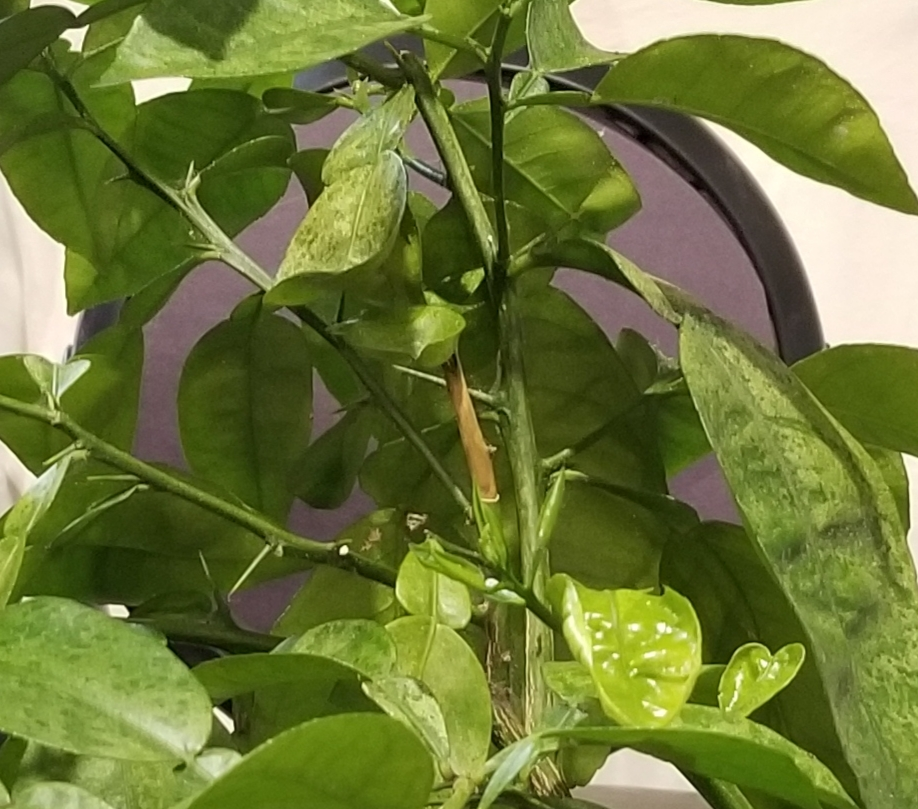
\includegraphics[width=0.33\columnwidth]{Fan.jpg}
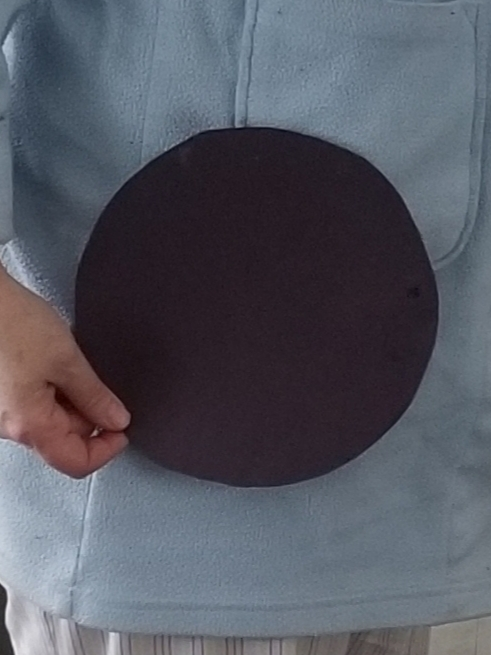
\includegraphics[width=0.33\columnwidth]{Fan1.jpg}
\end{center}
\caption{The exposed area of the fan-shaped construction paper with and without the plant in front of it.}
\label{fig:Appendix1}
\end{figure}


\begin{figure}
\begin{center}
\includegraphics[width=0.33\columnwidth]{MetalLeaf.jpg}
\includegraphics[width=0.33\columnwidth]{Paper.jpg}
\end{center}
\caption{The orange construction paper of known area photographed with and without the model leaf overlaid.}
\label{fig:Appendix2}
\end{figure}
\begin{table}
\begin{center}
Displacement (\si{in})\\
\begin{tabular}{cccc}
\toprule
grapefruit & grapefruit & grapefruit & metal leaf \\
speed 1 & speed 2 & speed 3 & speed 3(cm) \\ 
\midrule
0.397 & 0.635 & 0.794 & 0.200 \\
0.476 & 0.476 & 0.635 & 0.0500 \\
0.635 & 0.635 & 0.794 & 0.100 \\
0.476 & 0.556 & 0.794 & 0.200 \\
0.476 & 0.635 & 0.794 & 0.150 \\
\label{tb2:Table2}
\bottomrule
\end{tabular}
\end{center}
\end{table}

\end{document}
